\documentclass{article}
\usepackage{float}
\usepackage[a4paper, top=2.5cm, bottom=2.5cm, left=2.5cm, right=2.5cm]{geometry}
\usepackage[super,sort&compress]{natbib}
\bibliographystyle{unsrtnat}
\usepackage{textcomp}
\usepackage{graphicx}
\usepackage{authblk}
\usepackage{booktabs}

\title{
  Understanding Recovery from Malnutrition in Early Life:\\
  A Multi-Omic Analysis of the Infant Gut Microbiome, Plasma Lipidome, and Neurodevelopmental Outcomes
}

\author[1]{Authors}
%\author[1,*]{Theo Portlock}
%\author[2,*]{Talat Sharma}
%\author[2,*]{Shahria Hafiz Kakon}
%\author[3,*]{Berit Hartjen}
%\author[1,*]{Chris Pook}
%\author[1,*]{Brooke Wilson}
%\author[3]{Ayisha Bhuttor}
%\author[1]{Daniel Ho}
%\author[1]{Inoli Shennon Wadumesthrige Don}
%\author[3]{Anne-Michelle Engelstad}
%\author[3]{Renata Di Lorenzo}
%\author[3]{Garrett Greaves}
%\author[3]{Caroline Kelsey}
%\author[1]{Peter Gluckman}
%\author[1,4,5,6]{Justin O'Sullivan}
%\author[7]{Terrence Forrester}
%\author[3]{Charles Nelson}
%
\affil[1]{Affiliations}
%\affil[1]{The Liggins Institute, University of Auckland, NZ}
%\affil[2]{Infectious Diseases Division, International Centre for Diarrheal Disease Research, Bangladesh}
%\affil[3]{Department of Pediatrics, Boston Children’s Hospital and Harvard Medical School; Harvard Graduate School of Education, Boston, USA}
%\affil[4]{The Maurice Wilkins Centre, The University of Auckland, New Zealand}
%\affil[5]{MRC Lifecourse Epidemiology Unit, University of Southampton, UK}
%\affil[6]{Singapore Institute for Clinical Sciences, A*STAR, Singapore}
%\affil[7]{Faculty of Medical Sciences, UWI Solutions for Developing Countries, The University of the West Indies, Jamaica}
%\affil[*]{These authors contributed equally}

\date{}

\begin{document}

\maketitle

\tableofcontents

\newpage
\section{Abstract}
Recovery from undernutrition during childhood has historically centered on short term weight gain with little attention given to redressing the delays in neurocognitive development.
Herein we discuss the results of a prospective, randomized controlled trial for the use of an enhanced, brain-targeted micronutrient supplemented nutritional rehabilitation regimen versus the standard of care and healthy age-matched controls on measures of cognition and emotional regulation in a cohort of one-year-old Bangladeshi children.
This longitudinal, multimodal study explains biological mechanism through network analysis to understand the impacts of a dietary intervention.

\newpage
\section{Main}
% Definition of MAM
Malnutrition refers to deficiencies, excesses, or imbalances in a person’s intake of energy and/or nutrients and can refer to undernutrition, overweight, or obesity.
% Importance of MAM
Malnutrition is a global crisis (UN SDG2: Zero Hunger) \cite{UN_SDG2}.
% Why MAM and not SAM
Moderate Acute Malnutrition (MAM) is the most common, most treatable form of undernutrition.
% What does MAM do
MAM in childhood delays the development of multiple systems in the body from the gut microbiome to neurocognition.
% Treament rates
A small proportion of children with MAM are treated.
% What is treatment
Treatment involves refeeding.
% Problems with refeeding
Current Refeeding methods focus solely on short term weight gain, associate with serious adverse events (such as diarrhoea or Refeeding Syndrome), and are often ineffective at restoring developmental trajectories.
Those that recover their weight often have lasting neurological deficits including cognition and emotional regulation.
% Microbiome connection
MAM is associated with gut microbiome immaturity.
% Microbiome targetted refeeding
Novel prototypical refeeding methods, such as microbiota-directed complementary foods (MDCFs) target the gut-microbiome-brain axis as a mediator to address these deficits.
% Effectiveness of MCDF
By inoculating gnotobiotic pig and mice preclinical models with age-characteristic gut microorganisms, MDCFs increased the levels of biomarkers and mediators of growth, bone formation, neurodevelopment, and immune function toward a state resembling healthy children \cite{gehrig2019effects}.
% Need to improve on these methods
Developing these methods into sustainable refeeding strategies is needed urgently.
% The difficulty in predicting Recovery measurements
% Our study aims
Herein we discuss the results of a study that empoys The Enhanced Ready to Use Supplementary Food (E-RUTF) plus Small Quantity Lipid Based Nutrient Supplement (E-SQLNS) as compared to standard RUTF commonly used to treat childhood Moderate Acute Malnutrition (MAM) 

\section{Results}
\subsection{Study population characteristics}
% Why was Bangladesh picked
As a city with the second highest density of population and in a country with childhood malnutrition rate is one of the highest globally, the Mirpur region in Dhaka, Bangladesh was chosen to assess the impact of early-life malnutrition \cite{ahmed2012nutrition}.
% Number of children selected and when (marasmic vs kwashiokor wasn't defined)
% Recovery statistics (rates, days to recovery, and sustained recovery with biases measured) - \ref{Table1}. Complications (feeding failure, days of disease)
Refeeding resulted in recovery in approximately half the children with MAM, with no significant difference in rate between the two refeed methods (43.0\% in the Local RUSF group vs 41.2\% in the ERUSF group , MWU. p = 0.9460).
However, a key distinction emerged in time to recovery, which was shorter by approximately ten days in the ERUSF group (p = 0.0422, d = 0.46) (Table 1)

\begin{table}[h!]
	\centering
	\caption{Study population characteristics, sociodemographic information, comorbitities, and recovery rates}
	%\input{my_imported_table.tex}
	\label{Table1}
\end{table}

\begin{figure}[H]
	\centering
	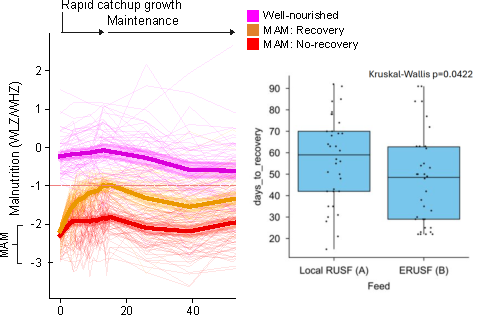
\includegraphics[scale=1.2]{figures/anthrochange_simple.pdf}
	\caption[Measures of cognition were not significantly impacted by refeeding]{
		Measures of cognition were not significantly impacted by refeeding.
		a) Lineplot of how children change in WLZ/WHZ during refeeding.
		b) Boxplot of days to recovery compared between the feeding groups.
	}
	\label{Figure1}
\end{figure}

\subsection{What influenced recovery}
% A background to the data collected
Acknowledging that the refeed type made little impact on the overall recovery rates, an investigation into the factors that were associated with anthropometric recovery was undertaken.
% risk factors for sustained recovery
% are the same factors important for reocvery rates/days to recovery/sustained recovery?
% Why mixed models - maaslin3

% Influence of anthropometrics on recovery
The most significant factors were anthropometric such as head circumference, indicating extent of malnutrition.
% Influence of genetics on recovery
%% Background on the PRS method
% Influence of behaviour on recovery
%% Introduce measurements (FCIS, Glitter wand, Spin the pots, PCI, PSS, Sleep, 
% Influence of socioeconomic environment on recovery
Other factors included the proportion of days without feeding failure, and comorbidites
% Influence of faecal microbiome on recovery
%% alpha diversity
%% beta diversity
%% species
%% functions
% Influence of plasma metabolites on recovery
%% AA
%% Vitamins

\subsection{What did recovery influence}
% Maaslin3

\subsection{Factors improved/deteriorated during the treatment}
% Definition of improvement
The classification of a given microbiome as 'healthy' has long been contested.
This is true also of a number of datasets within this cohort.
% Explaination of approach taken from the RDA version!
Thus, a method whereby the distance between the composition of the overall community of each dataset was compared with the respective well-nourished age-matched control for each timepoint.
For each dataset analysed through this technique, the shrinking/widening of this distance with respect to the well-nourished controls between the two timepoints was used to indicate improvement/deterioration.
% approach results
ERUTF drove a greater shift toward healthy microbiome, including depletion of \textit{S. wadsworthensis} and \textit{L. fermentum}.

\begin{figure}[H]
	\centering
	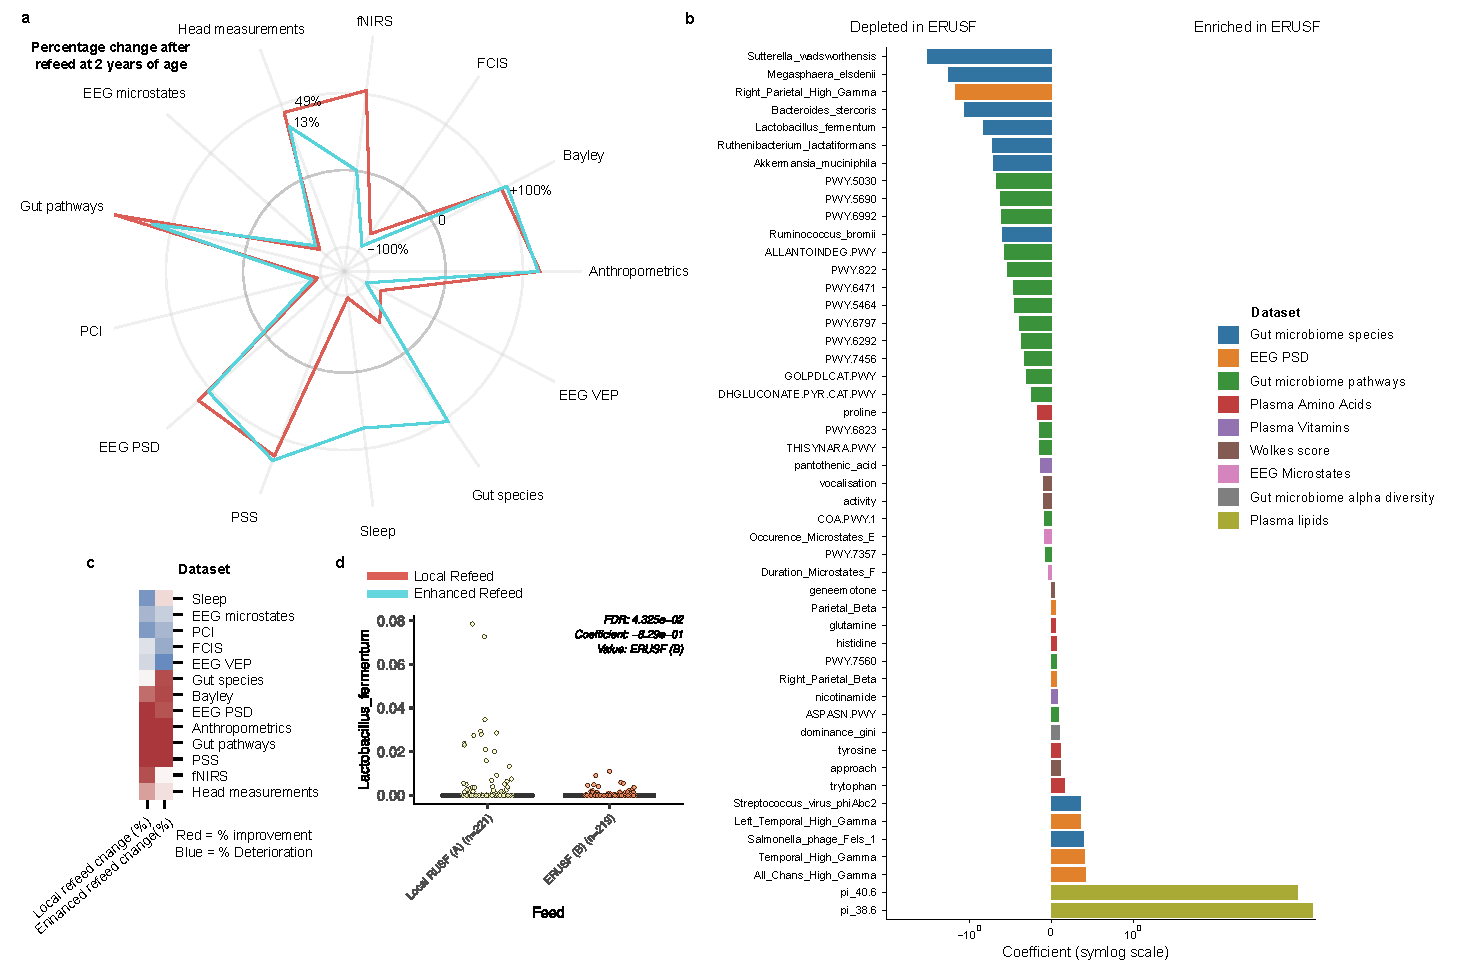
\includegraphics[scale=0.6]{figures/newrecoveryfeed3.pdf}
	\caption[Refeed methods improve/deteriorate bodily systems differently]{
		Refeed methods improve/deteriorate bodily systems differently.
		A, Radial plot of percentage change in distance from Well-nourished controls before and after refeeding (1yr and 2yr). Positive and negative percentages represent improvement and deterioration, respectively.
		B, Horizontal barplot of features that explain the change significantly (q \textless{} 0.2) between refeed methods after mixed modelling for each dataset.
		C, Heatmap to show clusters of dataset changes.
		D, Boxplot to show how Lactobacillus fermentum changes according to the refeed method.
	}
\label{Figure2}
\end{figure}

\subsection{Using a systems biology approach to understand recovery}
% Difficulties of interpretation of multiple datasets - including missing data
% MOFA and factorisation
% Machine learning pipeline explaination

\subsection{Network-Based Integration of Multimodal Changes to understand recovery mechanism}
% Networks as a tool to understand data relationships
% Limitations of causality
% How to link the results together
With an understanding of the impacts that the enhanced refeed method had on developmental trajectories across the datasets recoreded, the next step was to understand how those changes might be connected together mechanisticly.
% Network stats - number of nodes, edges, directional nodes, interaction effects
It was found that proline metabolism was correlated with EEG and cognitive outcomes, suggesting neuro-metabolic recovery pathways.

\begin{figure}[H]
\centering
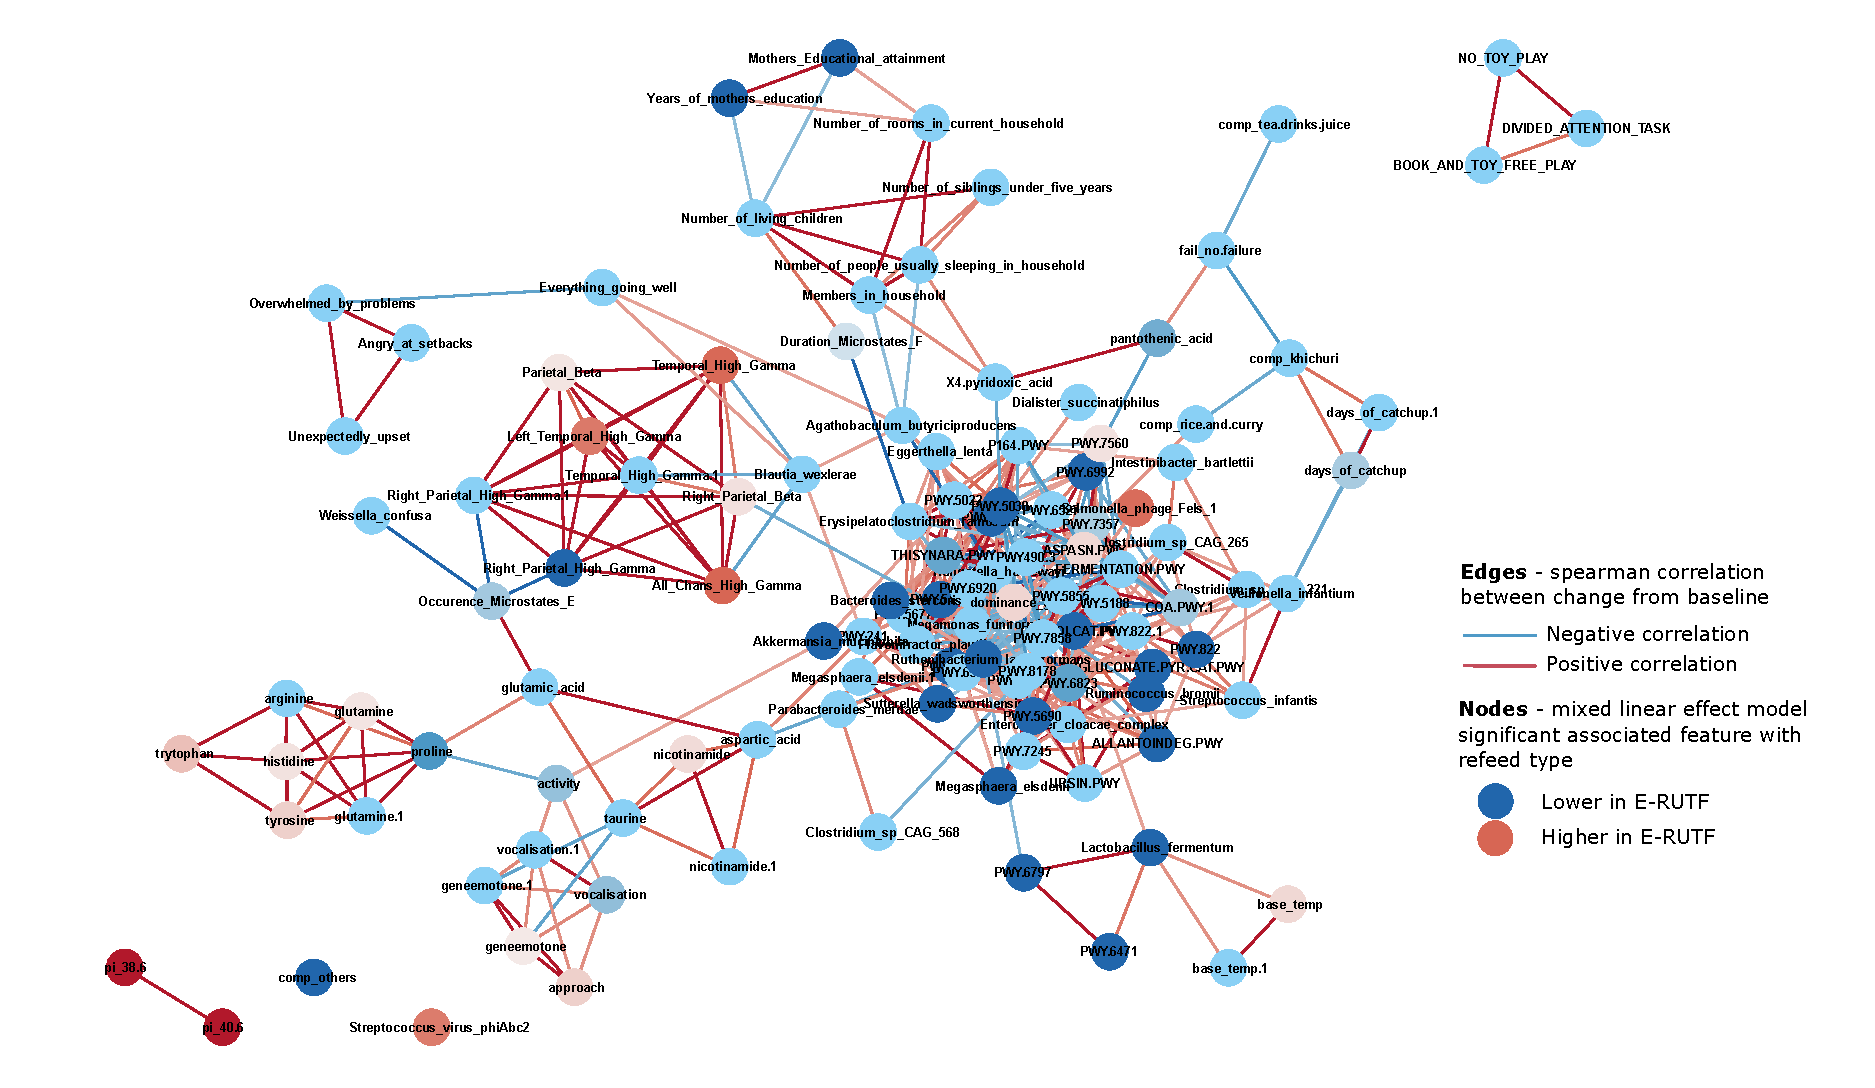
\includegraphics[scale=0.5]{figures/mixedmodelnetwork.pdf}
	\caption[Mechanism of E-RUTF differential impacts on brain structure]{
		Mechanism of E-RUTF differential impacts on brain structure.
	}
\label{Figure3}
\end{figure}

\section{Discussion}

\section{Conclusion}

\section{Methods}
PSS method \cite{mozumder2022reliability}

\subsection{Ethics}
The M4EFaD intervention was registered NCT05629624 on clinicaltrials.gov.
The study was approved by icddr,b Ethical Review Committee PR-21084 and the Bangladesh Directorate General of Drug Administration.
Ethical review for the analytical component was obtained from Auckland Health Research Ethics Committee approval AH23922 (metabolomics, metagenomics, machine learning).

\subsection{Study Design and Participants}
The study was performed on the baseline, and two year data from three cohorts of infants who were enrolled (between Jan – December 2022) as part of the M4EFaD intervention within the Mirpur slum, Dhaka, Bangladesh.
Inclusion criteria included a diagnosis of malnutrition, no history of chronic medical conditions, and no antibiotic use within the past month.

\subsection{Recruitment and anthropometric data collection}
Enrolment was initiated on February 7, 2022, and continued until February 2024.
Study surveillance workers (SWs) conducted a door-to-door census (approximately 100,000 households) in Mirpur DNCC wards ward 2, 3 and 5 between January and December 2022.
Verbal consent was obtained to participate in the census.
The census identified 5736 children aged between 11 to 13 months and 2,314 children aged between 34 to 38 months.
During the census, if the guardian verbally consented to the study procedure, and the babies met the inclusion and exclusion criteria of the study, the SWs proceeded to measure the MUAC of the child.
Mothers of babies who were within the MUAC range were invited to visit the icddr,b study clinic for further assessment and enrolment.
Final screening for eligibility and study consent occurred at the icddr,b Mirpur study clinic.
The consenting process was tailored to each mother's literacy level and involved reviewing the inclusion and exclusion criteria.
Comprehension of the study was assessed using scripted points and open-ended questions.
Following consent, the clinical screening team completed a screening form, capturing the date of enrolment, sex, date of birth (DOB), weight (in kg), length/ height (in cm), head circumference (in cm), and Mid-Upper Arm Circumference MUAC measurements of the child.
The WLZ/WHZ Z-score for each child was calculated using the WHO anthropometric calculator.
The child's age was validated using the EPI vaccination card.
Neurological measures, Bailey scores, EEG data were collected upon enrolment to evaluate neurological development.

\subsection{EEG data collection and analysis}
Continuous scalp EEG was recorded using NetStation 4.5.4. and 128-channel Hydrocel Geodesic Sensor Nets modified to remove eye electrodes (Electrical Geodesics, Inc. (EGI), Eugene, OR, USA).
Data was sampled at 500 Hz.
Impedances were kept under 100 k\textohm{} when possible and measured once at the beginning of the session, and again halfway through.
Sessions were conducted in a dimly lit room with the participants sitting on the parent’s lap.
The participants were separated from the research staff conducting the session by a curtain, but the testing area was not acoustically or electrically shielded.
A second research staff member was present in the testing area to help keep the participant engaged.
EEG sessions consisted of 6 paradigms, i.e., resting state, visual working memory, flanker, disengagement, visual evoked potential, and auditory stimuli.
The subsequent (pre-)processing steps were applied to the resting state data where participants watched a 3-minute video that featured toys.

EEG data were preprocessed offline with MatLab (R2021B) using the Harvard Automated Processing Pipeline for Electroencephalography (HAPPE) Version 3 (Gabard-Durnam et al., 2018).
A specified subset of 30 channels was excluded (‘E1’, ’E8’, ’E14’, ’E17’, ’E21’, ‘E25’, ’E32’, ‘E38’, ‘E43’, ’E44’,’ E48’, ’E49’, ’E56’, ’E63’, ’E68’, ’E73’, ’E81’, ’E88’, ’E94’, ’E99’, ’E107’, ’E113’, ’E114’, ’E119’, ’E120’, ’E121’, ‘E125', 'E126', 'E127', 'E128').
Data were downsampled to 250Hz, bandpass filtered (1-100Hz), and filtered using a 50Hz cleanline filter for line noise removal.
Bad channels were then automatically identified and rejected, and wavelet-enhanced Independent Component Analysis (ICA) and the Multiple Artifact Rejection Algorithm (MARA) were performed to detect and impute artifacts.
Resting state data were segmented into 2s epochs; epochs with an amplitude >±150mV were rejected.
Segments were also rejected using segment similarity criteria.
Data were then re-referenced to the average of all channels.

EEG outputs from HAPPE were then reformatted and processed using the Batch Electroencephalography Automated Processing Platform (BEAPP) (Levin et al., 2018) to extract power spectra for each participant across the following frequency bands: delta (2-4Hz), theta (4-6Hz), low alpha (6-9Hz), high alpha (9-12Hz), beta (12-30Hz), and gamma (30-45Hz) and the following regions of interest (see Supp Figure 2): occipital (‘E70’, ’E71’, ’E75’, ‘E76’, ‘E83’), temporal (‘E36’,‘E40’, ‘E41’, ‘E45’, ‘E46’, ‘E102’, ‘E103’, ‘E104’, ‘E108’, ‘E109’), parietal (‘E52’, ‘E53’, ‘E59’, ‘E60’, ‘E85’, ‘E86’, ‘E91’, ‘E92’), and frontal (‘E5’, ‘E6’, ‘E12’, ‘E13’, ‘E24’, ‘E27’, ‘E28’, ‘E33’, ‘E34’, ‘E112’, ‘E116’, ‘E117’, ‘E122’, ‘E123’, ‘E124’).
Further, PSD values were normalized by a Log\textsubscript{10} transform.

\subsection{Developmental Outcomes} 
The Bayley Scales of Infant and Toddler Development, Fourth Edition (BSID-IV) cognitive, language, and motor subscales were administered to all participants.
Research assistants were trained to research reliability in the administration and scoring of the Bayley-4.
Due to cultural differences between the Bangladesh and the United States where the assessment was developed, Bangladeshi researchers modified some assessment stimuli to improve cultural responsiveness and relevancy.
For example, pictures for the item naming series and action naming series of the expressive language and receptive language subscales were adapted to include items that Bangladeshi children are more likely to be familiar with and bedtime clothing that would signify the child in the picture was going to sleep instead of the one-piece pajamas worn in the original picture, which the Bangladeshi children would not be familiar with. 

\subsection{Biological sample collection}
Stool samples were collected from each infant at their home at the baseline visit.
Samples were collected in DNA/RNA Shield Fecal Collection Tubes (Zymo Research, \#R1101).
Peripheral venous blood samples were collected in EDTA Vacutainers, separated into plasma and RBCs and immediately frozen at -80 C.
Batches of blood and stool samples were air-freighted on dry ice from Bangladesh to the Liggins Institute, New Zealand for processing and analysis. 

\subsection{Microbiome DNA extraction and sequencing}
DNA was extracted from stool samples using the ZymoBIOMICS MagBead DNA/RNA extraction kit (Zymo Research, \#R2136) following the standard protocol.
Samples (1 mL) were mechanically lysed in bead bashing tubes using the MiniG tissue homogenizer prior to extraction of DNA.
200 µL of the sample was used post-bead bashing for extraction of DNA following the protocol.
A volume of 50 \textmu{} L of elute was collected in DNAse/RNAse Free Water.
Samples with a DNA concentration \textless{} 14.5 ng/\textmu{}L were re-extracted following the ZymoBIOMICS DNA extraction protocol.
Samples were sequenced (Illumina NovaSeq 150PE reads) to an average sequencing depth of 20M read-pairs/sample.
Raw sequences were processed using BioBakery3 tools \cite{beghini2021integrating}, specifically read quality filtering and human decontamination with KneadData (Version 1), taxonomic profiling with MetaPhlAn3 (Version 3.1, using the mpa\_v31\_CHOCOPhlAn\_201901 database) and functional profiling using presence/absence and abundance of microbial pathways (MetaCyc) with HUMAnN3 (Version 3.6).
A minimum threshold of \textgreater{} 0.1\% relative abundance and \textgreater{} 5\% prevalence for all detected species was applied. 

\subsection{Plasma lipidomics}
Plasma samples for lipidomics were thawed on ice and extracted according to a method modified from \citet{liu2016plasma}.
Briefly, 10 \textmu{}L volume was placed in an amber glass autosampler vial and 300 \textmu{}L of a mixture of Type 1 water, butanol, methanol, chloroform and SPLASH Lipidomix in a ratio of 4:15:15:20:1 was added.
The mixture was vortexed and sonicated at room temperature before the protein precipitate was removed by centrifugation and an aliquot of supernatant transferred to an amber glass autosampler for negative ionisation LC-MS/MS.
A second aliquot of supernatant was diluted 5 times with 75\% IPA for positive ionisation LC-MS/MS.
A 5 µL volume of each sample was injected onto a Phenomenex Kinetex F5 column (100 mm × 2.1 mm × 2.6 \textmu{}m) and lipids were separated using a ternary gradient of Type 1 water, methanol and isopropanol containing ammonium acetate.
Lipids were quantified and identified with a Q-Exactive mass spectrometer (Thermo Fisher Scientific, Germany) equipped with a heated electrospray ionisation HESI source.
Data was processed using MS-DIAL v4.92 92 \cite{tsugawa2015ms}.
For full methodological details see the supplementary information.

\subsection{Statistical Analyses}
Python version 3.9.2 was used to perform all analysis \cite{van1995python}.
Due to the unequal sample sizes and non-normally distributed data; non-parametric statistical approaches were used for differential abundance analysis.
Relative abundances were adjusted by Centred Log Ratio to account for the compositional nature of the dataset \cite{gloor2016s}.
Log adjusted fold change significance was measured using (MWU) test using the ‘mannwhitneyu’ function from ‘scipy.stats’ and adjusted for multiple testing using the ‘fdrcorrection’ function from statsmodels.stats.multitest.
PCoA ordinations (plotted using 'skbio.stats.ordination.pcoa' module) were used to visualise the clustering of the Bray-Curtis dissimilarities (calculated using skbio.distance.pdist) between samples from their species and functional composition.
To quantify the variance of the gut microbiome explained covariates, PERMANOVA p-values were calculated from those Bray-Curtis Dissimilarities using the ’permanova’ function from the 'skbio.stats.distance' module.
Bray-Curtis were also used to capture the temporal dynamics of the microbiome from baseline.
Numerical Associations between species and metadata were measured with Spearman correlation (calculated using 'spearmanr' function from 'scipy.stats' module), where significance was defined as FDR adjusted p-values of \textless{} 0.05 as per \citet{2020SciPyNMeth}.
Associations between categorical data were measured with Fisher's Exact test (calculated using 'fisher\_exact' from 'scipy.stats' module), where significance was defined as p-values of \textless{} 0.05.

\subsection{Machine learning}
SHAP Value (SHapley Additive exPlanations) interpretation was used to interpret the contributions each feature had on the model's performance using the ‘shap’ python package \cite{lundberg2017unified}.

\subsection{Network analysis}
Absolute spearman rho of above 0.3 were used as edges and gut bacterial species and functional profiles, EEG, and plasma lipids were used as nodes coloured by their mean SHAP scores for classifier models that distinguish MAM from well-nourished conditions.

\section{Code availability}
All analysis code is available on the GitHub repository.
The codebase is organised into scripts, providing a comprehensive framework for replicating the experiments.
Detailed documentation and instructions on how to use the code are provided in the repository's README file.

\section{Ethics approval and consent to participate}
Ethical approvals were obtained from the Research Review Committee (RRC; August 21, 2021) and Ethical Review Committee (ERC) of icddr,b (protocol no: PR-21084; September 21, 2021), Institutional Review Board of Boston Children’s Hospital, USA (for analyses of neuropsychological assessments), University of Auckland, New Zealand (approval AH23922; for analyses of collected biological samples) and University of West Indies (CREC-MN.51, 21/22).

\section{Data availability}
EEG and metadata are available from the authors, upon reasonable request that meets the ethics of the study.

\section{Competing interests}
The authors declare that they have no competing interests.

\section{Funding}
Work on this clinical trial is supported by Wellcome Leap (9942 Culver Blvd Unit 1277 Culver City, CA 90232-4167, United States; www.wellcomeleap.org) to PDG, JMO, TF and CAN as part of the 1kD Program.
We acknowledge our core donors, Governments of Bangladesh, Canada for providing unrestricted support and commitment to icddr,b's research effort.

\section{Author Contributions}
TP, KG and JOS drafted and co-wrote the manuscript.
TS, SHK, BCW, BH, CP, AB, DH, IS, AME, RD, GG, CK, PDG, RH, TF, CAN commented on the manuscript.
JMO, RH, TF, PDG, CAN designed the study and analyses.
TS, SHK performed assessments and obtained samples in Dhaka.
RH oversaw the Dhaka group.
TP performed multiomic analyses, BCW and IS performed metagenomics, CP performed metabolomics, JOS oversaw the Auckland group.
BH performed EEG analyses, CAN oversaw the Boston group.

\section{Acknowledgements}
The authors would like to acknowledge the participants in Mirpur, Dhaka, Bangladesh for their contributions to this study.
The authors would also like to thank the study team within the Infectious Diseases Division, International Centre for Diarrheal Disease Research, Bangladesh for their work in participant recruitment, sample collection and assessments.

\bibliography{writing/manuscript/library}

\newpage

\section{Supplementary material}
\begin{figure}[!htb]
\centering
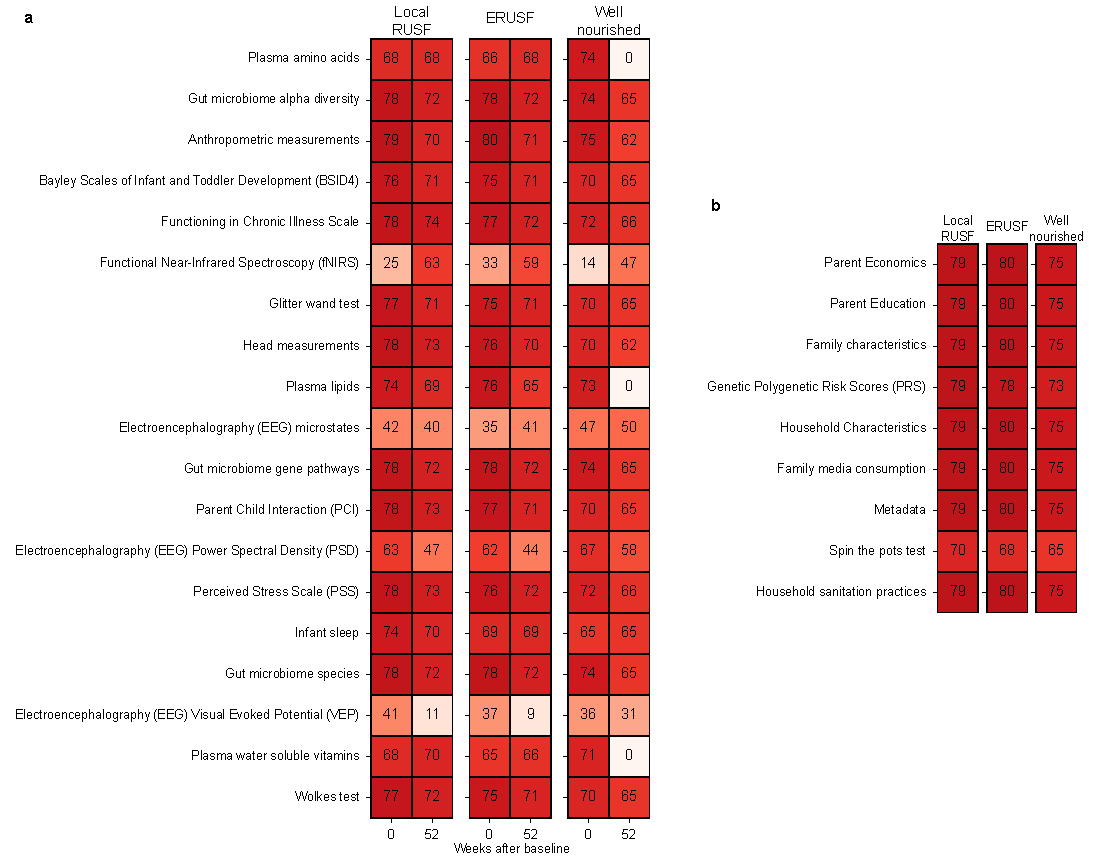
\includegraphics[scale=0.8]{figures/newalldata.pdf}
	\caption[Datasets recoreded in the M4EFaD study]{
		Datasets recorded in the M4EFaD study.
	}
\label{Figure1}
\end{figure}

\end{document}
